%DO NOT MESS AROUND WITH THE CODE ON THIS PAGE UNLESS YOU %REALLY KNOW WHAT YOU ARE DOING
\chapter{Introduction} \label{Introduction}

\section{Preamble} \label{Preamble}
\noindent Compared to other biometric features such as the iris and fingerprint. There are inherent advantages of Gait such as it is perceivable at a distance, it need not be in contact and it is non-invasive. It works on itself without any user cooperation. Another important aspect is that it gives readings under low light conditions which is fairly accurate. Also disguising, hiding one’s gait or imitating some other person’s gait is practically impossible. As a result it has fascinated several security-sensitive environments such as classified research and nuclear labs, military, banks etc. Gait recognition is particularly useful in crime scenes where other biometric traits (such as face or fingerprint) might be obscured intentionally. 

\noindent Two common categories of gait recognition are appearance-based and model-based approaches. Among the two, the appearance-based approaches suffer from changes in the appearance owing to the change of the viewing or walking directions. Model based ones are view and scale invariant and reflect in the kinematic characteristics of walking manner. In this study we present a model based approach using the Microsoft Kinect sensor which offers us a 3D model of the human skeleton with capability to track up to 25 joints of the human body. 
\section{Motivation}\label{Motivation}
\noindent The initial motivation to build a gait recognition system developed after watching the Gait Analysis scene in the movie Mission Impossible – Rogue Nation (2015) where it was used for authentication for security purposes. Although at that time it felt as a futuristic technology, through research we realised that existing gait recognition approaches mostly use standard video cameras for capturing and recording the movement of walking persons. Here, the main difficulty lies in the extraction of characteristic features that can be used for identification. The challenges of existing gait recognition system and the possibilities Kinect offers lead to the assumption that the problem of gait recognition could be simplified using the Kinect sensor.
\newpage

\section{Proposed Idea} \label{Proposed Idea}
\noindent In this paper we propose a skeleton model based approach (provided by Microsoft Kinect Sensor) for gait recognition and person identification. Our system consists of three components: The first component records the skeletal data offered by Kinect using the SDK provided by Microsoft. The second component processes on this data using MATLAB for feature extraction. Finally we use different classification algorithms available in MATLAB classification toolbox to identify a person using previously recorded training data and compare their performance and accuracy. This is a prototypic implementation of a gait recognition system, where we evaluate the possibilities of gait recognition using the Microsoft Kinect.

\begin{figure}[H]
\centering 
{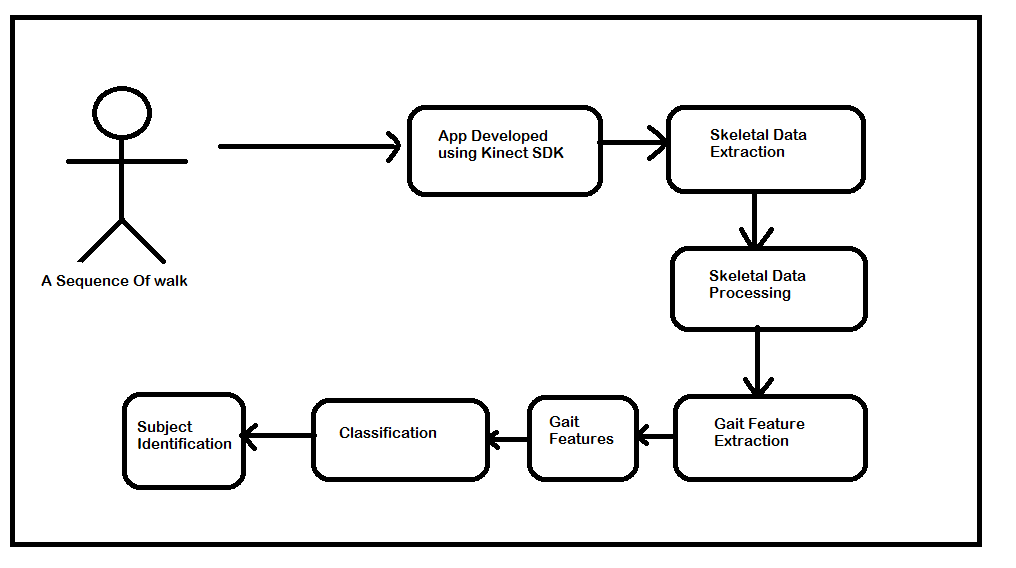
\includegraphics[scale=0.55]{Figprocessflow.png}}
\caption{Process flow diagram}
\end{figure}

